%!TEX TS-program = pdflatex
% dissertation.tex -- main dissertation file
%
% Wisconsin dissertation template
% Copyright (c) 2008-2009 William C. Benton.  All rights reserved.
%
% This program can redistributed and/or modified under the terms
% of the LaTeX Project Public License Distributed from CTAN
% archives in directory macros/latex/base/lppl.txt; either
% version 1 of the License, or (at your option) any later version.
%
% This program includes other software that is licensed under the
% terms of the LPPL and the Perl Artistic License; see README for details.
%
% You, the user, still hold the copyright to any document you produce
% with this software (like your dissertation).
%

%%% You'll want ``oneside'' for the deposit version, but probably not for any versions that don't need to meet the UW requirements
\documentclass[12pt,oneside,letterpaper]{memoir}

% preamble.tex -- packages to include
%
% Wisconsin dissertation template
% Copyright (c) 2008 William C. Benton.  All rights reserved.
%
% This program can redistributed and/or modified under the terms
% of the LaTeX Project Public License Distributed from CTAN
% archives in directory macros/latex/base/lppl.txt; either
% version 1 of the License, or (at your option) any later version.
%
% This program includes other software that is licensed under the
% terms of the LPPL and the Perl Artistic License; see README for details.
%
% You, the user, still hold the copyright to any document you produce
% with this software (like your dissertation).

%% You should use natbib
\IfFileExists{natbib.sty}{%
\usepackage{natbib}%
}{}

%% You probably need appendix, if you want appendices
\IfFileExists{appendix.sty}{%
\usepackage{appendix}%
}{}

%% the spacing in memoir is weird, you'll need to use this
\DisemulatePackage{setspace}
\usepackage[onehalfspacing]{setspace}

%% geometry package to help with margins on title page
\usepackage{geometry}

%% List setup; the ``hanglist`` environment will allow you to have
%% nicely-typeset enumerated lists (i.e. with the numbers hanging in
%% the margins).  You need at least version 2.1 of enumitem.sty.  If
%% you don't have enumitem installed at all, hanglist will just be an
%% alias for enumerate.
\IfFileExists{enumitem.sty}{%
\usepackage[loadonly]{enumitem}[2007/06/30]%
\newlist{hanglist}{enumerate}{1}%
\setlist[hanglist]{label=\arabic*.}%
\setlist[hanglist,1]{leftmargin=0pt}%
}{%
\newenvironment{hanglist}{\begin{enumerate}}{\end{enumerate}}%
}

%% Comment out any of these that you don't want
\usepackage{amssymb}
\usepackage{amsmath}
\usepackage{amsthm}
%\usepackage{theorem}
\usepackage{hyperref}

\IfFileExists{mathpartir.sty}{%
\usepackage{mathpartir}%
}{}

%%%%% LISTINGS package and setup
\IfFileExists{listings.sty}{%
\usepackage{listings}%
}{}



%% Get rid of ugly borders around PDF hyperlinks (e.g. for cross-references, bib entries, or URLs)
\hypersetup{pdfborder = 0 0 0}

%% You want microtype.
\IfFileExists{microtype.sty}{%
\usepackage[protrusion=true,expansion=true]{microtype}%
}{}

%\pagestyle{thesisdraft}

% Surround parts of graphics with box
\usepackage{boxedminipage}

%% booktabs (thx to Nate Rosenblum for bringing this beautiful package
%% to my attention)
\IfFileExists{booktabs.sty}{%
\usepackage{booktabs}%
}{}

% This is now the recommended way for checking for PDFLaTeX:
\usepackage{ifpdf}

%% Avoid ugly "Type 3" fonts
\usepackage{lmodern}
\usepackage[LY1]{fontenc}

%% Substitute your favorite serif and sans fonts here....
\IfFileExists{tgpagella.sty}{%
% TeX Gyre pagella, like Palatino
\usepackage{tgpagella}%
}{}

\usepackage[LY1]{eulervm}

\ifpdf
\usepackage[pdftex]{graphicx}
\else
\usepackage{graphicx}
\fi

% Tomislav's packages:
\usepackage{multirow}
\usepackage{rotating}
\usepackage{makecell}
\usepackage{xcolor}

\usepackage{makeidx}
\makeindex

{\theoremstyle{plain}
\newtheorem{thm}{Theorem}[chapter]
\newtheorem{cor}[thm]{Corollary}
\newtheorem{define}[thm]{Definition}
\newtheorem{exmpl}[thm]{Example}
}
{\theoremstyle{remark}
\newtheorem{rmk}[thm]{Remark}
}

\newtheoremstyle{customsty1}
{3pt}%
{3pt}%
{}% --- body font
{}% --- indent amount
{\bfseries}% --- Theorem head font
{:}% --- Punctuation after head
{.5em}% --- space after head
{}% --- theorem head spec (can be left empty, meaning 'normal')

% Define 'newtheorems' that use ``customsty1''
{\theoremstyle{customsty1}
}


%%% NB: the ``deposit'' chapter- and page- styles should conform to UW
%%% requirements.  If you are producing a pretty version of your
%%% dissertation for web use later, you will certainly want to make
%%% your own chapter and page styles.

\makechapterstyle{deposit}{%
  \renewcommand{\chapterheadstart}{}
  \renewcommand{\printchaptername}{}
  \renewcommand{\chapternamenum}{}
  \renewcommand{\printchapternum}{\parbox{2em}{\MakeLowercase{\Large\scshape\thechapter{}}} }
  \renewcommand{\afterchapternum}{}
  \renewcommand{\printchaptertitle}[1]{%
  \raggedright\Large\scshape\MakeLowercase{##1}}
  \renewcommand{\afterchaptertitle}{%
  \vskip\onelineskip \hrule\vskip\onelineskip}
}

\makepagestyle{deposit}

\makeatletter

\renewcommand{\chaptermark}[1]{\markboth{#1}{}}
\renewcommand{\sectionmark}[1]{\markboth{#1}{}}

\makeevenfoot{deposit}{}{}{}
\makeoddfoot{deposit}{}{}{}
\makeevenhead{deposit}{\thepage}{}{}
\makeoddhead{deposit}{}{}{\thepage}
\makeatother

%%% set up page numbering for chapter pages to satisfy UW requirements
%%% NB: You will want to delete until the ``SNIP'' mark if you are
%%% making a ``nice'' copy
\copypagestyle{chapter}{plain}
\makeoddfoot{chapter}{}{}{}
\makeevenhead{chapter}{\thepage}{}{}
\makeoddhead{chapter}{}{}{\thepage}
%%% SNIP

%%% bib nonsense
\makeatletter
\newenvironment{wb-bib}[1]{%
  \chapter*{references}
\ifnobibintoc\else
\phantomsection
\addcontentsline{toc}{chapter}{References}
\fi
\prebibhook
  \begin{bibitemlist}{#1}}{\end{bibitemlist}\postbibhook}

\AtBeginDocument{%
  \@ifpackageloaded{natbib}{% natbib is loaded
    \addtodef{\endthebibliography}{}{\vskip-\lastskip\postbibhook}
    \@ifpackagewith{natbib}{sectionbib}{% with sectionbib option
      \renewcommand{\bibsection}{\@memb@bsec}}%
      {\renewcommand{\bibsection}{\@memb@bchap}}}%
  {}
  \@ifpackagewith{chapterbib}{sectionbib}{%
    \renewcommand{\sectionbib}[2]{}
    \renewcommand{\bibsection}{\@memb@bsec}}{}
}
\makeatother

% defs.tex -- wbepi environment for chapter epigraphs and other useful defs.
%
% Wisconsin dissertation template
% Copyright (c) 2008 William C. Benton.  All rights reserved.
%
% This program can redistributed and/or modified under the terms
% of the LaTeX Project Public License Distributed from CTAN
% archives in directory macros/latex/base/lppl.txt; either
% version 1 of the License, or (at your option) any later version.
%
% This program includes other software that is licensed under the
% terms of the LPPL and the Perl Artistic License; see README for details.
%
% You, the user, still hold the copyright to any document you produce
% with this software (like your dissertation).


%% put lstnewenvironment declarations here, if you're using listings

%% end lstnewenvironment declarations

%% I put convenience definitions that will go in several chapters here

%%%%% begin convenience definitions

\makeatletter
\newcommand{\wb@episource}{}
\newenvironment{wbepi}[1]{\begin{quote}\renewcommand{\wb@episource}{#1}\itshape}{\par\upshape \raggedleft --- \textsc{\wb@episource}\\ \end{quote}}
\makeatother

%%%%% SVN
\IfFileExists{svn-multi.sty}{%
\usepackage{svn-multi}%
%%% Uncomment the second one and comment out the first one if you want
%%% to include subversion revision information in each file.
\newcommand{\vcinfo}{}%
%\newcommand{\vcinfo}{\begin{centering}\fbox{\fbox{\parbox{5in}{Author: \svnauthor\\Revision: \svnfilerev\\Last changed on: \svnfiledate\\URL: \svnkw{HeadURL}}}}\\[1em]\end{centering}}%
}{%
\newcommand{\svnidlong}[4]{}%
\newcommand{\svnfilerev}{}%
\newcommand{\svnauthor}{}%
\newcommand{\svnfiledate}{}%
\newcommand{\svnkw}{}%
\newcommand{\vcinfo}{}%
}

%%%%% end convenience definitions

% thesisdefs.tex

% This is mostly adapted from withesis.cls.  The original copyright
% notice for withesis.cls follows, preceded by two percent signs (%%):

%% withesis.cls
%% LaTeX Style file for the University of Wisconsin-Madison Thesis Format
%% Adapted from the Purdue University Thesis Format
%% Originally by Dave Kraynie
%% Edits by Darrell McCauley
%% Adapted to UW-Madison format by Eric Benedict  (Noted with <EB>)
%% Updated to LaTeX2e by Eric Benedict 24 July 00
%%
%%=============================================================================
%% Licensed under the Perl Artistic License.
%% see: http://www.ctan.org/tex-archive/help/Catalogue/licenses.artistic.html
%% for more info...
%%=============================================================================

% withesis.cls is available from CTAN.  The modifications to this file
% are also licensed under the Perl Artistic License.

% --wb, 2008

\makeatletter

\newcounter {tocpage}
\newcounter {lofpage}
\newcounter {lotpage}
\newcounter {listofheading}

\newcommand\@thesistitlemedskip{0.25in}
\newcommand\@thesistitlebigskip{0.55in}
\newcommand{\degree}[1]{\gdef\@degree{#1}}
\newcommand{\project}{\gdef\@doctype{A masters project report}}
\newcommand{\prelim}{\gdef\@doctype{A preliminary report}}
\newcommand{\thesis}{\gdef\@doctype{A thesis}}
\newcommand{\dissertation}{\gdef\@doctype{A dissertation}}
\newcommand{\department}[1]{\gdef\@department{(#1)}}
\newcommand{\oralexamdate}[1]{\gdef\@oralexamdate{#1}}
\newcommand{\committeeone}[1]{\gdef\@committeeone{#1}}
\newcommand{\committeetwo}[1]{\gdef\@committeetwo{#1}}
\newcommand{\committeethree}[1]{\gdef\@committeethree{#1}}
\newcommand{\committeefour}[1]{\gdef\@committeefour{#1}}
\newcommand{\committeefive}[1]{\gdef\@committeefive{#1}}
\newcommand{\committeesix}[1]{\gdef\@committeesix{#1}}
\newcommand{\committeeseven}[1]{\gdef\@committeeseven{#1}}

\newenvironment{titlepage}
 {\@restonecolfalse\if@twocolumn\@restonecoltrue\onecolumn
  \else \newpage \fi \thispagestyle{empty}
% \c@page\z@ -- deleted: count title page in thesis
}{\if@restonecol\twocolumn \else \newpage \fi}

\gdef\@degree{Doctor of Philosophy}    %Default is PhD
%\gdef\@doctype{A dissertation}         %Default is dissertation
\gdef\@doctype{A preliminary report}         %Default is dissertation

\gdef\@department{(Computer Sciences)} % Default is Electical Engineering
\gdef\@oralexamdate{}
\gdef\@committeeone{}
\gdef\@committeetwo{}
\gdef\@committeethree{}
\gdef\@committeefour{}
\gdef\@committeefive{}
\gdef\@committeesix{}
\gdef\@committeeseven{}



\renewcommand{\maketitle}{%
  \begin{titlepage}
%-----------------------------------------------------------------------------
% -- The thesis office doesn't like thanks on title page.  Put it in
% -- the acknowledgments.  This is here so you don't have to change
% -- your titlepage when converting from report style. -> from Purdue, but I
%        left it here since it seems compatible with UW-Madison, Eric
%-----------------------------------------------------------------------------
    \def\thanks##1{\typeout{Warning: `thanks' deleted from thesis titlepage.}}
    \let\footnotesize\small \let\footnoterule\relax \setcounter{page}{1}
 %sets new margins for title page so that committee members can be placed there

   % \vspace*{0.1in}
    \begin{center}
      {\textbf{\expandafter\uppercase\expandafter{\@title}}} \\[\@thesistitlebigskip]
       by \\[\@thesistitlemedskip]
      \@author \\[\@thesistitlebigskip]
      %\@doctype\ submitted in partial fulfillment of \\
      %the requirements for the degree of\\[\@thesistitlebigskip]
      %\@degree \\[\@thesistitlemedskip]
      %\@department \\[\@thesistitlebigskip]
      %at the \\[\@thesistitlebigskip]
      Department of Computer Sciences\\
      University of Wisconsin--Madison\\[\@thesistitlebigskip]
      Preliminary Dissertation Report\\[\@thesistitlebigskip]
      \@date \\[\@thesistitlebigskip]
    \end{center}
% section added by Steven Baumgart on 3/2012
% adds committee list to the title page
% add or delete committee members as you need to, these are defined in the dissertation.tex document
% comment out other things as you need to as well. - SB

%\noindent Date of final oral examination: \@oralexamdate \hspace*{\fill} \\[\@thesistitlemedskip]
%\noindent The dissertation is approved by the following members of the Final Oral Committee:\\*
\noindent \textbf{Committee:}\\*
\indent \@committeeone\\*
\indent \@committeetwo\\*
\indent \@committeethree\\*
\indent \@committeefour\\*
\indent \@committeefive
%\indent \@committeesix\\* %if you uncomment any of these you the last line needs to have no line break ``//*``
%\indent \@committeeseven


  \end{titlepage}

  \setcounter{footnote}{0}
  \setcounter{page}{1} %title page is NOT counted
  \let\thanks\relax
  \let\maketitle\relax \let\degree\relax \let\project\relax \let\prelim\relax
  \let\department\relax
  \gdef\@thanks{}\gdef\@degree{}\gdef\@doctype{}
  \gdef\@department{}
  %\gdef\@author{}\gdef\@title{}
}


%=============================================================================
% ABSTRACT
%=============================================================================
% The abstract should begin with two single-spaced lines describing
% the author and title in a standard format.  After these lines comes
% the standard abstract.
%=============================================================================
\def\abstract{
  \chapter*{Abstract}
  \addcontentsline{toc}{chapter}{Abstract}
  \relax\markboth{Abstract}{Abstract}}
\def\endabstract{\par\newpage}


%=============================================================================
% UMI ABSTRACT
%=============================================================================
% The UMI abstract should begin with the author and title in a standard format.
% After the author comes the advisor and university. After these lines comes
% a bunch of double spaced text to make up the standard abstract.
% After the abstract, the advisor's approval signature follows.
% This page is not numbered and is delivered seperately to the thesis office.
%=============================================================================

\def\advisortitle#1{\gdef\@advisortitle{#1}}
\def\advisorname#1{\gdef\@advisorname{#1}}
\gdef\@advisortitle{Professor}
\gdef\@advisorname{Cheer E.\ Place}

\def\umiabstract{
             \thispagestyle{empty}
                  \addtocounter{page}{-1}
                \begin{center}
                  {\textbf{\expandafter\uppercase\expandafter{\@title}}}\\
                  \vspace{12pt}
                  \@author \\
                  \vspace{12pt}
                  Under the supervision of \@advisortitle\ \@advisorname\\
                  At the University of Wisconsin-Madison
                \end{center}
}

\def\endumiabstract{\vfill \hfill\@advisorname\par\newpage}


%============================================================================
% VERBATIMFILE
%============================================================================
% \verbatimfile{<filename>}    for verbatim inclusion of a file
% - Note that the precise layout of line breaks in this file is important!
% - added the \singlespace - EB
%============================================================================
\def\verbatimfile#1{\begingroup \singlespace
                    \@verbatim \frenchspacing \@vobeyspaces
                    \input#1 \endgroup
}


%=============================================================================
% SEPARATOR Pages
%   Creates a blank page with a text centered horizontally and vertically.
%   The page is neither counted nor numbered.
%   These pages are required in the thesis format before sections such
%   as appendices, vita, bibliography, etc.
%=============================================================================
\def\separatorpage#1{
  \newpage
  \thispagestyle{empty}
  \addtocounter{page}{-1}
  \null
  \vfil\vfil
  \begin{center}
    {\textbf{#1}}
  \end{center}
  \vfil\vfil
  \newpage}


%=============================================================================
% COPYRIGHTPAGE
%=============================================================================
% The copyright must do the following:
% - start a new page with no number
% - place the copyright text centered at the bottom.
%=============================================================================
\def\copyrightpage{
  \newpage
  \thispagestyle{empty}    % No page number
  \addtocounter{page}{-1}
  \chapter*{}            % Required for \vfill to work
  \begin{center}
   \vfill
   \copyright\ Copyright by \@author\ \@date\\
   All Rights Reserved
  \end{center}}


%=============================================================================
% GLOSSARY
%=============================================================================
% The glossary environment must do the following:
% - produce the table of contents entry for the glossary
% - start a new page with GLOSSARY centered two inches from the top
%=============================================================================
\def\glossary{
  \chapter*{GLOSSARY}
  \addcontentsline{toc}{chapter}{Glossary}}
\def\endglossary{\par\newpage}

%=============================================================================
% NOMENCLATURE
%=============================================================================
% The nomenclature environment must do the following:
% - produce the table of contents entry for the nomenclature section
% - start a new page with NOMENCLATURE centered two inches from the top
%=============================================================================
\def\nomenclature{\separatorpage{DISCARD THIS PAGE}
  \chapter*{Nomenclature}
  \addcontentsline{toc}{chapter}{NOMENCLATURE}}
\def\endnomenclature{\par\newpage}

%=============================================================================
% CONVENTIONS
%=============================================================================
% The conventions environment must do the following:
% - produce the table of contents entry for the nomenclature section
% - start a new page with CONVENTIONS centered two inches from the top
%=============================================================================
\def\conventions{\separatorpage{DISCARD THIS PAGE}
  \chapter*{Conventions}
  \addcontentsline{toc}{chapter}{CONVENTIONS}}
\def\endconventions{\par\newpage}


%=============================================================================
% COLOPHON
%=============================================================================
% The colophon environment must do the following:
% - produce the table of contents entry for the nomenclature section
% - start a new page with COLOPHON centered two inches from the top
%=============================================================================
\def\colophon{\separatorpage{DISCARD THIS PAGE}
  \chapter*{Colophon}
  \addcontentsline{toc}{chapter}{Colophon}}
\def\endcolophon{\par\newpage}

%=============================================================================
% LIST OF SYMBOLS
%=============================================================================
% The list of symbols environment must do the following:
% - produce the table of contents entry for the list of symbols section
% - start a new page with LIST OF SYMBOLS centered two inches from the top
%=============================================================================
\def\listofsymbols{\separatorpage{DISCARD THIS PAGE}
  \eject
  \chapter*{LIST OF SYMBOLS}
  \addcontentsline{toc}{chapter}{LIST OF SYMBOLS}}
\def\endlistofsymbols{\par\newpage}

%=============================================================================
% VITA
%=============================================================================
% The vita environment must do the following:
% - produce a separator page with the word vita centered
% - produce the table of contents entry for the vita
% - start a new page with VITA centered two inches from the top
%=============================================================================
\def\vita{
%  \separatorpage{VITA}         % UW doesn't require this EB
  \chapter*{VITA}
  \addcontentsline{toc}{chapter}{VITA}}
\def\endvita{\par\newpage}

%=============================================================================
% ACKNOWLEDGMENTS
%=============================================================================
% The acknowledgments environment must do the following:
% - start a new page with ACKNOWLEDGMENTS centered two inches from the top
%=============================================================================
\def\acks{
  \chapter*{Acknowledgments}
}
\def\endacks{\par\newpage}

%=============================================================================
% DEDICATION
%=============================================================================
% The dedication environment must do the following:
% - start a new page
% - center the text vertically
% - include the text in a center environment
%=============================================================================
\def\dedication{
  \newpage
  \null\vfil
  \begin{center}}
\def\enddedication{\end{center}\par\vfil\newpage}

%=============================================================================
% DATE
%=============================================================================
%\def\today{\ifcase\month\or
  %January\or February\or March\or April\or May\or June\or
  %July\or August\or September\or October\or November\or December\fi
  %\space\number\day, \number\year}
\newcount\@testday
\def\today{\@testday=\day
  \ifnum\@testday>30 \advance\@testday by -30
  \else\ifnum\@testday>20 \advance\@testday by -20
  \fi\fi
  \number\day\ \
  \ifcase\month\or
    January \or February \or March \or April \or May \or June \or
    July \or August \or September \or October \or November \or December
    \fi\ \number\year
}


%  Single counter for theorems and theorem-like environments:
\newtheorem{theorem}{Theorem}[chapter]
\newtheorem{assertion}[theorem]{Assertion}
\newtheorem{claim}[theorem]{Claim}
\newtheorem{conjecture}[theorem]{Conjecture}
\newtheorem{corollary}[theorem]{Corollary}
\newtheorem{definition}[theorem]{Definition}
\newtheorem{example}[theorem]{Example}
\newtheorem{figger}[theorem]{Figure}
\newtheorem{lemma}[theorem]{Lemma}
\newtheorem{prop}[theorem]{Proposition}
\newtheorem{remark}[theorem]{Remark}

%=============================================================================
% TABLE OF CONTENTS; LIST OF FIGURES; LIST OF TABLES
%=============================================================================
% In report style, \tableofcontents, \listoffigures, etc. are always
% set in single-column style.  @restonecol is used to keep track of
% whether we need to switch back to double column style after the toc.
%
% The only known problem now is that the first page with the new
% layout is too long.  The problem seems to be that the change to
% textheight doesn't take place on the first page.  Even if it's the
% first line in the table of contents macro.  Presumably the same
% problem also occurs in the lof and lot.
%
% I'm taking a shot at fixing the problem by dropping in a throw-away
% page between the change to the height parameters and the start of
% the chapter.  Isn't elegance wonderful?
%
%=============================================================================

% \def\@tableof#1#2#3#4#5{
% { % limit scope of following declarations!!
%   \@restonecolfalse\if@twocolumn\@restonecoltrue\onecolumn\fi
%   \addtolength{\textheight}{-40pt}       % -24-16
%   \addtolength{\majorheadskip}{-40pt}    % -24-16
%   \addtolength{\headheight}{52pt}        %  36+16
%   \addtolength{\headsep}{-12pt}          % -12
%   \separatorpage{DISCARD THIS PAGE}
%   \chapter*{#1}
%   #5
%   \relax\markboth{#1}{#1}
%   \hbox to \hsize{#2 \hfil Page}
%   \singlespace
%   \setcounter{#3}{0}
%   \setcounter{listofheading}{1}  % change from 0 to 1 by mccauley, 14may93
%   \def\@oddhead{\vbox to \headheight{\vspace{4pt}
%     \hbox to \hsize{\hfil\textrm{\thepage}} \vfil
%     \ifnum\value{#3}=1
%       \ifnum\value{listofheading}=2
%         \hbox to \hsize{Appendix\hfil} \vspace{4pt} \fi
%       \ifnum\value{listofheading}=1
%         \stepcounter{listofheading} \fi
%       \hbox to \hsize{#2 \hfil Page}
%     \else
%       \setcounter{#3}{1}
%     \fi}}
%   \def\@evenhead{\vbox to \headheight{\vspace{4pt}
%     \hbox to \hsize{\textrm{\thepage}\hfil} \vfil
%     \ifnum\value{#3}=1
%       \ifnum\value{listofheading}=2
%         \hbox to \hsize{Appendix\hfil} \vspace{4pt} \fi
%       \ifnum\value{listofheading}=1
%         \stepcounter{listofheading} \fi
%       \hbox to \hsize{#2 \hfil Page}
%     \else
%       \setcounter{#3}{1}
%     \fi}}
%   \@starttoc{#4}  \if@restonecol\twocolumn\fi
%   \newpage
% }}
%
% \def\tableofcontents{\@tableof{TABLE OF CONTENTS}{}{tocpage}{toc}{}}
%
% \def\listoffigures{
%   \@tableof{LIST OF FIGURES}{Figure}{lofpage}{lof}
%   {\protect\addcontentsline{toc}{chapter}{LIST OF FIGURES}}}
%
% \def\listoftables{
%   \@tableof{LIST OF TABLES}{Table}{lotpage}{lot}
%   {\protect\addcontentsline{toc}{chapter}{LIST OF TABLES}}}

%=============================================================================
% BIBLIOGRAPHY
%=============================================================================
% The thebibliography environment executes the following commands:
%
%  o start a new 'chapter' with BIBLIOGRAPHY as the heading
%  o produce a separator page for the bibliography
%
%  \def\newblock{\hskip .11em plus .33em minus -.07em} --
%      Defines the `closed' format, where the blocks (major units of
%      information) of an entry run together.
%
%  \sloppy  -- Used because it's rather hard to do line breaks in
%      bibliographies,
%
%  \sfcode`\.=1000\relax --
%      Causes a `.' (period) not to produce an end-of-sentence space.
%=============================================================================
% \altbibtitle
%   The default title for the References chapter is ``LIST OF REFERENCES''
%   Since some people prefer ``BIBLIOGRAPHY'', the command
%   \altbibtitle has been added to change the chapter title.
%   This command does nothing more than change REFERENCES to BIBLIOGRAPHY
%============================================================================
\def\@bibchaptitle{Bibliography}
\def\altbibtitle{\def\@bibchaptitle{Bibliography}}
\def\thebibliography#1{
  %\separatorpage{\@bibchaptitle}
  \global\@bibpresenttrue
  \chapter*{\@bibchaptitle\markboth{\@bibchaptitle}{\@bibchaptitle}}
  \addcontentsline{toc}{chapter}{\@bibchaptitle}
  \vspace{0.375in}    % added to match 4 line requirement
  \interlinepenalty=10000 % added to prevent breaking of bib entries
  \singlespace\list
  {[\arabic{enumi}]}{\settowidth\labelwidth{[#1]}\leftmargin\labelwidth
    \advance\leftmargin\labelsep \usecounter{enumi}}
  \def\newblock{\hskip .11em plus .33em minus -.07em}
  \sloppy
  \sfcode`\.=1000\relax}
\let\endthebibliography=\endlist



\makeatother


\clearpage\pagenumbering{roman}  % This makes the page numbers Roman (i, ii, etc)

\title{Effective Directed Gaze for Character Animation}
\author{Tomislav Pejsa}
\department{Computer Sciences}
\oralexamdate{8/5/15}
\committeeone{Professor Michael Gleicher, co-chair (\textit{University of Wisconsin--Madison})}
\committeetwo{Professor Bilge Mutlu, co-chair (\textit{University of Wisconsin--Madison})}
\committeethree{Professor Kevin Ponto, (\textit{University of Wisconsin--Madison})}
\committeefour{Professor Eftychios Sifakis, (\textit{University of Wisconsin--Madison})}
%\committeefive{Professor Adriana Tapus, (\textit{ENSTA ParisTech})}

% if you use any additional committe members you will need to uncomment
% the corresponding lines 107 and/or 108 in thesisdef.tex You may also need
% to adjust the value for \newcommand\@thesistitlemedskip{0.25in} and
% \newcommand\@thesistitlebigskip{0.55in} in line 32 to get it to all fit
%\committeesix{Iam A. Professor, Associate Professor, Geography}
%\committeeseven{Iam A. Professor, Professor, Computer Sciences}


\date{August 5, 2015}

\begin{document}

%%% Uncomment the following if your .bib contains references that you will not
%%% explicitly cite, but that should be in the final bibliography:
% \nocite{*}

\ifpdf
\DeclareGraphicsExtensions{.pdf, .jpg, .tif}
\else
\DeclareGraphicsExtensions{.eps, .jpg}
\fi

\newgeometry{left=1in,right=1in,bottom=1in,top=1in}
\maketitle
\restoregeometry %sets the margins back to normal

%% Add \part declarations if you want, but it's not necessary
%\part{Preliminaries}

%%% SOME OF THIS CODE IS ADAPTED FROM THE VENERABLE withesis.cls

% COPYRIGHT PAGE
%  - To include a copyright page use \copyrightpage
%\copyrightpage

% DEDICATION
%\begin{dedication}
%	\emph{Please insert your dedication here.}
%\end{dedication}

%% BEGIN PAGESTYLE

%%% You can pick a pagestyle if you want; see the memoir class
%%% documentation for more info.  The default ``deposit'' option meets
%%% the UW thesis typesetting requirements but is probably
%%% unsatisfactory for making a version of your dissertation that
%%% won't be deposited to the graduate school (e.g. for web or a nice
%%% printed copy)

\chapterstyle{deposit}
\pagestyle{deposit}


% ACKNOWLEDGMENTS
%\begin{acks}
%\begin{wbepi}{David C.~Makinson (1965)}
It is customary for authors of academic books to include in their prefaces statements such as this: ``I am indebted to ... for their invaluable help; however, any errors which remain are my sole responsibility.'' Occasionally an author will go further. Rather than say that if there are any mistakes then he is responsible for them, he will say that there will inevitably be some mistakes and he is responsible for them....

Although the shouldering of all responsibility is usually a social ritual, the admission that errors exist is not --- it is often a sincere avowal of belief. But this appears to present a living and everyday example of a situation which philosophers have commonly dismissed as absurd; that it is sometimes rational to hold logically incompatible beliefs.
\end{wbepi}

Above is the famous ``preface paradox,'' which illustrates how to use the \texttt{wbepi} environment for epigraphs at the beginning of chapters.  You probably also want to thank the Academy.
%\end{acks}

% CONTENTS, TABLES, FIGURES
\renewcommand{\printtoctitle}[1]{\chapter*{#1}}
\renewcommand{\printloftitle}[1]{\chapter*{#1}}
\renewcommand{\printlottitle}[1]{\chapter*{#1}}

\renewcommand{\tocmark}{}
\renewcommand{\lofmark}{}
\renewcommand{\lotmark}{}

\renewcommand{\tocheadstart}{}
\renewcommand{\lofheadstart}{}
\renewcommand{\lotheadstart}{}

\renewcommand{\aftertoctitle}{}
\renewcommand{\afterloftitle}{}
\renewcommand{\afterlottitle}{}

\renewcommand{\cftchapterfont}{\normalfont}
\renewcommand{\cftsectionfont}{\itshape}
\renewcommand{\cftchapterpagefont}{\normalfont}
\renewcommand{\cftchapterpresnum}{\bfseries}
\renewcommand{\cftchapterleader}{}
\renewcommand{\cftsectionleader}{}
\renewcommand{\cftchapterafterpnum}{\cftparfillskip}
\renewcommand{\cftsectionafterpnum}{\cftparfillskip}

% \captionnamefont{\small\sffamily}
% \captiontitlefont{\small\sffamily}

\renewcommand{\contentsname}{Contents}
% \renewcommand{\listfigurename}{list of figures}
% \renewcommand{\listtablename}{list of tables}

\tableofcontents

%\clearpage
%\listoftables

%\clearpage
%\listoffigures

\clearpage
% NOMENCLATURE
% \begin{conventions}
% % \begin{description}
% % \item{\makebox[0.75in][l]{term}
% %        \parbox[t]{5in}{definition\\}}
% % \end{description}
% \input{conventions}
% \end{conventions}

%\advisorname{Bilge Mutlu}
%\advisortitle{Professor}
% ABSTRACT
\begin{abstract}
  In order to perform effectively as virtual actors, teachers, trainers, and storytellers, animated characters need to utilize \emph{directed gaze}---coordinated eye, head, and body movements toward a new focus of attention---to capture and manage the viewers' attention, directing it toward important objects and information and triggering high-level processes such as engagement and learning. The goal of my research is to make it easier for animators to produce directed gaze animation that looks visually plausible for the current scenario and is effective as a mechanism for attention management, engagement, and learning. My work will consist of developing and empirically evaluating a novel approach for authoring effective directed gaze animation, that will be robust to the character's body motion, morphology, and environment layout, and cost-effective with respect to authoring time and required expertise. In the proposed approach, directed gaze will be represented as a sequence of \emph{gaze shifts} toward specific targets; techniques will be provided for automated inference and manual editing of gaze behaviors based on this representation. The components of the work will be the following: (1) a procedural animation model for synthesis of individual gaze shifts; (2) techniques for automated adaptation of gaze shift motion to virtual characters with non-realistic and non-human morphologies; (3) an approach for authoring \emph{plausible} directed gaze animation, consisting of automated inference from body motion and environment and an accessible tool for manual editing; (4) an extension of the approach to support automated inference of \emph{effective} gaze that achieves animator-specified communicative goals; (5) a study with human participants evaluating the effectiveness of synthesized gaze animation on a virtual agent in a teaching scenario. 
\end{abstract}

%\begin{abstract}
%  In order to perform effectively as virtual actors, teachers, trainers, and storytellers, animated characters need to utilize \emph{directed gaze}---coordinated eye, head, and body movements toward a new focus of attention---to capture and manage the viewers' attention, directing it toward important objects and information and triggering high-level processes such as engagement and learning. The goal of my research is to make it easier for animators to produce directed gaze animation that looks visually plausible for the current scenario and is effective as a mechanism for attention management, engagement, and learning. My work will consist of developing and empirically evaluating a novel approach for authoring effective directed gaze animation, that will be robust to the character's body motion, morphology, and environment layout, and cost-effective with respect to authoring time and required expertise. In the proposed approach, directed gaze will be represented as a sequence of \emph{gaze shifts} toward specific targets; techniques will be provided for automated inference and manual editing of gaze behaviors based on this representation. The components of the work will be the following: (1) a procedural animation model for synthesis of individual gaze shifts; (2) techniques for automated adaptation of gaze shift motion to virtual characters with non-realistic and non-human morphologies; (3) an approach for authoring \emph{plausible} directed gaze animation, consisting of automated inference from body motion and environment and an accessible tool for manual editing; (4) an extension of the approach to support automated inference of \emph{effective} gaze that achieves animator-specified communicative goals; (5) a study with human participants evaluating the effectiveness of synthesized gaze animation on a virtual agent in a teaching scenario. 
%\end{abstract}

\clearpage\pagenumbering{arabic}

%%% END STUFF TAKEN FROM WITHESIS EXAMPLE FILE


%% Now include the tex files for each chapter, like so (I put these in separate dirs):
%%% SOME OF THIS CODE IS ADAPTED FROM THE VENERABLE withesis.cls

%% BEGIN PAGESTYLE

%%% You can pick a pagestyle if you want; see the memoir class
%%% documentation for more info.  The default ``deposit'' option meets
%%% the UW thesis typesetting requirements but is probably
%%% unsatisfactory for making a version of your dissertation that
%%% won't be deposited to the graduate school (e.g. for web or a nice
%%% printed copy)

\chapterstyle{deposit}
\pagestyle{deposit}

\chapter{Introduction}

Animated characters need to communicate effectively with humans, whether as cartoon actors in animated films or as animated teachers and storytellers giving virtual presentations, lectures, and task demonstrations. One important capability required for effective communication in these contexts is \emph{directed gaze}. I define directed gaze as coordinated movement of the eyes, head, and body toward target objects or information in the environment. People use directed gaze to indicate the focus of their attention to others, which facilitates a range of social and cognitive processes. For example, teachers and storytellers can gaze upon their audience to make the presentation more immediate, engaging, and instructive~\citep{fullwood2006effect,sherwood1987facilitative,otteson1980effect}. People can use gaze to redirect the attention of others to objects and information in the environment through the mechanism of \emph{joint attention}~\citep{dentremont2007early}. The ability to cue attention using gaze enables high-level meaning to be communicated more effectively during interactions---people ground linguistic references to objects by looking at them~\citep{hanna2007speakers,preissler2005role} and gaze also serves as a predictor of their intention to perform physical actions~\citep{strabala2012learning}. Well-animated gaze of a cartoon character or virtual agent can achieve the same effects. Professional animators expend much effort into animating believable gaze movements that capture the audience's attention and direct it toward the most important thing on the screen, while in the area of human-agent interaction, a growing number of studies~\citep{andrist2012designing,andrist2013aversion,mutlu2006storytelling} suggest that animated agents with appropriately designed gaze behavior perform better in educational and socially assistive roles.

Animating directed gaze that successfully fulfills these communicative functions is a challenging problem. A necessary, but insufficient requirement for gaze animation is that it must look \emph{plausible}---the character's gaze must look like something a human might do in the same situation, without unnaturalness and visual artifacts that might distract from what the character is communicating.
%Professional animators strive for "lifelike", "believable"... - character looks and behaves like a sentient being with personality, emotions, goals...
%That is a much higher bar and not one we strive to achieve - we care about enabling specific communicative effects that make the character good at its task (teaching, storytelling, training...) and not about creating a simulacrum of human life
Furthermore, gaze animation must be \emph{effective}---it must achieve communicative effects specified by the animator. Effective gaze is able to direct the viewer's attention, engage them, and help them understand the character's intents. The effectiveness of gaze is empirically verifiable by means of studies with human participants. Finally, the process of producing gaze animation must be \emph{robust} and \emph{cost-effective}. While a skilled animator might be able to hand-author plausible and effective gaze for a particular animated scenario, that approach is neither robust nor cost-effective---animation production using traditional keyframing tools requires considerable expertise and labor, and the resulting animation is specific to the current scenario and not robust to changes in the character's morphology, actions, and virtual environment. Motion capture is a robust solution for body animation, but not for gaze---a typical motion capture setup does not capture eye movements and results usually need to be hand-edited after the fact. Methods for automated synthesis of gaze animation (surveyed in Section~\ref{sec:BackgroundGazeAnimation}) are limited in different ways: they may apply only to a specific context (e.g., just conversational gaze) or specific types of gaze movements (e.g., just the eyes and head, but no body), they do not consider the problem of combining gaze with the (potentially complex and varied) body motion, they may not afford sufficient parametric control or manual editing support to achieve the desired communicative effect, and their effectiveness is often not validated empirically.

My thesis is that plausible, effective directed gaze animation can be produced in a robust and cost-effective way using an authoring approach based on automated, parametrically controlled synthesis and augmented by manual editing. The key idea of my approach is to represent directed gaze as a sequence of \emph{gaze annotations}, where each annotation concisely describes a gaze shift toward a single target (which can be an environment object or the camera.) Given an animated scenario with a character performing a sequence of actions (encoded in its body motion) within a virtual environment, the proposed approach will automatically infer a gaze annotation sequence describing a \emph{plausible} gaze behavior. The approach will allow for accessible manual editing of the gaze behavior by editing the annotation sequence. To achieve \emph{effective} gaze, the behavior inference model will expose attention parameters allowing the animator to specify the types of gaze patterns that will occur in the output behavior and achieve specific communicative effects. Given the annotation sequence, corresponding gaze shift movements will be synthesized using a procedural model of human gaze shift kinematics, adapted to the character's morphology, and layered onto the original body motion. The proposed approach will be \emph{robust} to variations in character morphology, body motion, environment layout, and communicative goals, as well as \emph{cost-effective} in requiring minimal expertise and many fewer editing operations than traditional keyframing to produce equivalent results.

My work will consist of developing the technical components of the approach and evaluations of its robustness, cost-effectiveness, as well as plausibility and effectiveness of the resulting gaze animation. Each of the components will constitute a distinct contribution. Technical components of the work will include: (1) a model for synthesis of individual \emph{directed gaze shifts} supporting coordinated eye, head, and torso movements; (2) \emph{stylized gaze} techniques for adaptation of gaze shift movements to non-realistic and non-human character morphologies; (3) an approach for authoring \emph{plausible gaze}, consisting of an automated gaze inference model, a manual editing tool, and techniques for layering gaze animation onto body motion; (4) an extension of this approach to support automated inference of \emph{effective} gaze that achieves animator-specified communicative effects. In addition, my work will include (5) an \emph{evaluation}, in a study with human participants, of the effectiveness of authored gaze behaviors on a virtual agent giving physical task demonstrations. Besides serving as an evaluation, this study will inform the design of virtual agents' gaze behaviors that make them more effective in the roles of teachers, trainers, and storytellers, and as such it will constitute a distinct contribution.

The focus of my work is on gaze animation in \emph{non-interactive} scenarios, where the character acts out a script and does not respond to input from the viewer. However, I hypothesize that the approach will generalize to the gaze of characters in interactive scenarios, such as characters and avatars in games and embodied conversational agents interacting with users in ``serious'' applications. The approach will operate on fairly generic, low-level inputs---captured (or hand-animated) body motion, 3D modeled environment, virtual camera, and a few optional, animator-specifiable parameters---and produce a similarly generic output---gaze animation. Such features are commonplace in wide range of interactive systems.
% TODO: get rid of this, or say it elsewhere, in fewer words

In the remainder of this document, I give a review of related work, followed by an overview of the components of my research. For each component, I will provide a discussion of its relevance to my thesis, overview of its technical implementation, and a plan for its evaluation.
%%% SOME OF THIS CODE IS ADAPTED FROM THE VENERABLE withesis.cls

%% BEGIN PAGESTYLE

%%% You can pick a pagestyle if you want; see the memoir class
%%% documentation for more info.  The default ``deposit'' option meets
%%% the UW thesis typesetting requirements but is probably
%%% unsatisfactory for making a version of your dissertation that
%%% won't be deposited to the graduate school (e.g. for web or a nice
%%% printed copy)

\chapterstyle{deposit}
\pagestyle{deposit}

\chapter{Related Work}

\section{Gaze in Human Communication}
\label{sec:BackgroundHumanGaze}

The ability to follow another person's gaze and infer the direction of their attention emerges in the first year of life \citep{scaife1975infant}. Following another person's gaze enables establishment of reference \citep{dentremont2007early}, inference of intent \citep{mumme2007actions}, and engagement in joint attention with the person \citep{dentremont2007early}. Joint attention facilitates learning and comprehension by associating speech utterances with objects and information in the environment. This ability also develops at an early age and is crucial for the acquisition of language \citep{woodward2005infants}. In dialogue, moving the eyes closely in step with a speaker allows the listener to use spatial structure to organize information in the same way as the speaker \citep{richardson2005looking}. Addressees also make use of the speaker's gaze as a cue for disambiguating references \citep{hanna2007speakers,preissler2005role}. Conversational partners' shared gaze toward referents is higher while they speak about those objects \citep{bard1988referring}.

Humans infer other people's direction of attention by integrating information about their eye gaze direction, head orientation \citep{hietanen1999does}, and body orientation \citep{langton2000eyes,hietanen2002social,pomianowska2011socialcues}. Changes in body orientation occur relatively rarely during interaction compared to gaze shifts involving eye and head movements and indicate larger shifts in attention and mutual involvement \citep{kendon1973visible,schegloff1998bodytorque}. People tend to reorient their bodies to avoid head rotations larger than 90$^{\circ}$ when gazing at someone \citep{kendon1973visible}. Changes in body orientation also occur when a new party joins a conversation in order to reconfigure the conversational formation \citep{kendon2010spacing}.

People are particularly sensitive to the gaze of others \citep{argyle1976gaze}. This is interpreted as being attended to and, depending on the context of interaction, can lead to either discomfort from feeling observed or genuine social interaction \citep{argyle1976gaze}. A person who makes increased eye contact is associated with greater perceived dynamism, likeability, and believability \citep{beebe1976effects}. These people are also seen as being more truthful or credible \citep{argyle1976gaze}. Studies have shown that that people who spend more time gazing at their conversational partner receive higher socioemotional evaluations \citep{goldberg1969visual}, while gaze aversion produces consistently negative effects in impressions of attraction, credibility, and relational communication \citep{burgoon1986communicative}.

Gaze is a significant contributor to \emph{immediacy}---the degree of perceived physical or psychological closeness between people \citep{mehrabian1966immediacy}. Students from primary school through college have been shown to learn better when they are gazed at by the lecturer \citep{burgoon1986communicative, fry1975effects, sherwood1987facilitative, otteson1980effect}. Learning in these cases was usually measured by the students' performance on recall tasks. In a similar study, gazing into the camera during a video link conversation was shown to increase the recall of the viewer at the other end \citep{fullwood2006effect}. Gaze's positive effect on recall is usually attributed to its role as an arousal stimulus, which increases attentional focus and therefore enhances memory \cite{kelley1988effects}.

\section{Gaze in Computer Animation}
\label{sec:BackgroundGazeAnimation}

Prior work in gaze animation is broadly surveyed in~\citep{ruhland2015gazereview} and has largely focused on the automated synthesis of natural gaze behavior given certain input information. I distinguish between \emph{low-level} models for gaze synthesis, which generate kinematics of gaze movements from a specification of where the character should be looking, and \emph{high-level} models, which determine \emph{where} to look based on high-level information. My proposed approach relates to prior work in both categories.

\subsection{Low-level Gaze Synthesis}

One of the most important eye movements in gaze is the \emph{saccade}---fast eyeball movement between fixations. Much of the prior work in gaze animation has focused on synthesis of natural saccadic gaze using statistical models learned from recorded eye movements~\cite{deng2005automated,le2012live,lee2002eyes}. Saccades are integral components of larger gaze shifts, where they occur in coordination with head and upper body movements. Researchers have proposed several models of eye-head coordination in gaze ~\cite{peters2010animating,lance2010expressive,andrist2012headeye}. These models expose parameters for controlling how much the head should turn toward the target over the course of the gaze shift, allowing a degree of control over head posture. They achieve motion naturalness in different ways. The Expressive Gaze Model~\cite{lance2010expressive} makes use of recorded motion data to add expressiveness to gaze movements, while the model by~\citet{andrist2012headeye} is procedural but uses kinematics derived from neurophysiological measurements of gaze. The data-driven model by~\citet{ma2009natural} is notable because it infers natural eye movements from motion-captured head movements. In my research, I propose a gaze inference and synthesis approach that does not infer eye movements directly; rather, we infer a high-level specification from which the overall gaze movement can be synthesized.

Several gaze synthesis models also incorporate coordinated torso movements~\citep{thiebaux2009realtime,lance2010expressive,heck2007automated,grillon2009crowds}. The model by~\citet{heck2007automated} is data-driven---turning of the torso is achieved by blending example torso postures. ~\citet{grillon2009crowds} use an inverse kinematics approach to adapt the body posture toward the target. ~\citet{thiebaux2009realtime} is the only model that affords parametric control over eye, head, and torso coordination, at the expense of naturalness.  The key feature of our model is the use of neurophysiology-based gaze kinematics, which ensure plausible movement quality across the model's parameter range.

\subsection{High-level Gaze Synthesis}

High-level gaze synthesis is concerned with synthesizing gaze behavior with respect to high-level perceptual, emotional, cognitive, and social competencies of the character. Visual attention models determine where the character should be looking based on visual features of the environment~\citep{peters2003attention}. Examples include models of idle gaze in interactive virtual environments~\citep{khullar2001look,cafaro2009animating,grillon2009crowds}, which help situate the character in the environment and make them appear more lifelike. Another category of models synthesize gaze behavior to signal the character's emotions and cognitive state. ~\citet{queiroz2007automatic} and ~\citet{lance2010expressive} have analyzed gaze in animated films and derived models for synthesis of emotionally expressive gaze. ~\citet{lance2007emotionally} have explored layering emotionally expressive content onto coordinated head and torso movements in gaze. Other researchers have proposed models for generating patterns of eye movements parametrized by emotional~\citet{li2012emotional} and cognitive~\citet{lee2007rickel} states of the character.

%Gaze is an important nonverbal cue in human conversations and a large body of work in gaze synthesis deals with synthesis of conversational gaze for virtual agents conversing with humans. Researchers have explored synthesis of gaze patterns that match the current conversational state~\cite{pelachaud2003modelling,masuko2007headeye}, gaze cues as nonverbal feedback while the agent is listening to the user~\cite{gratch2007rapport}, mutual gaze during storytelling to improve the agent's social presence~\cite{bee2010gaze}, averted gaze to regulate conversational turns and express cognitive state~\cite{andrist2013aversion}, gaze driven by prosodic and semantic features of speech~\cite{zoric2011oncreating,le2012live,marsella2013virtual}, etc. In the field of multimodal interaction, researchers have proposed systems for synthesis of coordinated nonverbal behaviors---such as gaze---from text annotations; examples include BodyChat~\cite{vilhjalmsson1998bodychat}, BEAT~\cite{cassell1999fully}, Spark~\cite{vilhjalmsson2004animating}, and systems based on Behavior Markup Language (BML)~\cite{vilhjalmsson2007bml}.
Gaze is an important nonverbal cue in human interaction, and a large body of work in gaze synthesis deals with synthesis of conversational gaze for virtual agents interacting with humans. Many effects of gaze in human-human interaction (Section~\ref{sec:BackgroundHumanGaze}) have also been observed in interaction with virtual agents and social robots. A virtual agent can employ gaze as an attention cue and assist people in localizing task-relevant objects in the environment~\citet{bailly2010gaze}. Mutual gaze during storytelling can improve the agent's social presence~\cite{bee2010gaze} and facilitate greater recall of the story~\citet{mutlu2006storytelling}. Virtual agent's head posture during gaze has significant effects on the interaction~\citet{andrist2012designing}---when the agent aligns its head more with the camera, it is perceived as more engaging, trustworthy, and likeable, while greater head alignment with task objects in the environment facilitates better recall of those objects. 
%%% SOME OF THIS CODE IS ADAPTED FROM THE VENERABLE withesis.cls

%% BEGIN PAGESTYLE

%%% You can pick a pagestyle if you want; see the memoir class
%%% documentation for more info.  The default ``deposit'' option meets
%%% the UW thesis typesetting requirements but is probably
%%% unsatisfactory for making a version of your dissertation that
%%% won't be deposited to the graduate school (e.g. for web or a nice
%%% printed copy)

\chapterstyle{deposit}
\pagestyle{deposit}

\chapter{Research Overview}

%The goal of my research is to enable animators to easily author directed gaze animation for virtual characters that looks plausible and communicates effectively. I propose a robust, cost-effective approach that is based on the idea of representing the gaze behavior as a sequence of gaze shifts and providing techniques for automated synthesis and easy manual editing of this sequence. The components of the work are: (1) a procedural, parametric model for synthesis of individual gaze shifts; (2) stylized gaze techniques for adapting gaze shift motion to a range of character designs; (3) authoring approach for obtaining plausible directed gaze for an input body motion and environment; (4) an extension to this approach for authoring effective directed gaze that satisfies animator-specified communicative goals; (5) a study with human participants evaluating the effectiveness of authored gaze behaviors in the context of task demonstrations with a virtual agent. I give an overview of each component in the following sections.

\section{Animating Directed Gaze Shifts (completed)}
\label{sec:GazeShifts}

I define a directed \emph{gaze shift} as a coordinated movement of the character's eyes, head, and torso toward a target in the environment, which is followed by a \emph{gaze fixation} of the target. In my approach, gaze shifts serve as building blocks of larger gaze patterns that achieve specific communicative effects. The first step of my research was then to enable animation of individual gaze shifts. To that end, we have developed a procedural, parametric model for gaze shift synthesis. Originally developed as an eye-head coordination model by~\citet{andrist2012headeye}, we have further extended it with support for coordinated upper body movement. The model is implemented as a procedural, dynamic, feed-forward animation controller that synthesizes rotational motion of the eyes, head, and torso joints toward the target using a set of kinematic laws derived from studies of primate gaze in neurophysiology~\citep{guitton1987gaze,mccluskey2007monkeys}. The use of neurophysiology-based kinematics enables the model to synthesize gaze motion that looks \emph{plausible}, while retaining the key advantage of procedural models---high degree of control.

The gaze shift model accepts as input the properties of the gaze shift that should be synthesized, which include gaze target location (3D point in space where the agent will look) and head and torso
\emph{alignment parameters}. The latter parameters specify how far each of these body parts will rotate relative to the target. For example, low head alignment specifies that the character should only minimally turn its head toward the target and look at it ``out of the corner of the eye'', whereas high head alignment means the character will face the target straight on (Figure~\ref{fig:HeadTorsoAlignment}). The idea of alignment parameters is to enable the animator to control the character's attention signal: by turning its head and torso more toward a target, the character communicates a higher level of attention toward the target. The ability to parametrically control how the gaze shift communicates attention is a key to creating \emph{effective} directed gaze. The intuitive gaze parametrization also makes the model \emph{cost-effective} with respect to animator effort and skill, because the animator does not need to worry about the timing of eye, head, and torso movements.

\begin{figure*}
\centering
\includegraphics[width=1\textwidth]{figures/HeadTorsoAlignment.pdf}
\caption{Examples of gaze shifts synthesized using our model: (1) The agent maintaining eye contact with the viewer. (2) Gaze shift to the side with low value of the head alignment parameter. (3) Gaze shift in the same direction, but with high head alignment value. (4) Gaze shift in the same direction with a small shift in torso posture. (5) As before, but with a large shift in torso posture.}
\label{fig:HeadTorsoAlignment}
\end{figure*}

\subsection{Evaluation}

The original head coordination model was evaluated in prior work~\citep{andrist2012headeye,andrist2012designing}, demonstrating its \emph{plausibility} (measured as perceived naturalness of observed gaze shifts~\citep{andrist2012headeye}) and communicative \emph{effectiveness} (measured respectively as accuracy of participants' guesses at the character's attention direction~\citep{andrist2012headeye} and the effects of head alignment on information recall, engagement, and subjective perceptions of the character~\citep{andrist2012designing}.)

Following our extensions of the model to torso movements, we conducted another evaluation measuring the effects of torso alignment. In the study, we had a virtual character perform a series of gaze shifts toward gaze targets (paintings) in its virtual environment with varying levels of torso alignment (Figure~\ref{fig:TorsoAlignStudyConditions}). For each set of paintings, the participants were asked to rate how interested the character appeared to be in each painting---perceived interest serving as a measure of the strength of torso orientation as an attention cue. Results showed that the more the character aligned its torso with a particular painting, the more interested she was perceived to be in that painting, thereby demonstrating the model's \emph{effectiveness}.

\begin{figure*}
\centering
\includegraphics[width=0.85\textwidth]{figures/TorsoAlignStudyConditions.pdf}
\caption{Conditions in the evaluation of our gaze shift model.}
\label{fig:TorsoAlignStudyConditions}
\end{figure*}

\section{Stylized Gaze (completed)}
\label{sec:StylizedGaze}

Gaze shift models such as the one developed in my own work (Section~\ref{sec:GazeShifts}) produce plausible gaze motion because they are based on the kinematics of real human gaze. As such, they implicitly incorporate biomechanical and neurophysiological constraints of the human visuomotor system. Applying these models to characters with non-humanlike designs, such as stylized characters found in animated films, would result in gaze motion that contains anomalous and distracting visual artifacts---in other words, it would no longer look \emph{plausible}. However, the ability to animate the gaze of stylized characters is important: stylization affords a way to emphasize and exaggerate the character's personality traits, enhance their appeal, and avoid uncanny valley effects that can occur in realistically designed characters~\citep{geller2008overcoming}. A \emph{robust} animation approach should be able to handle such varied character designs.

As part of this research thread, we identified visual artifacts that occur when animating characters with stylized designs with neurophysiologically accurate movements synthesized by our gaze shift model (Section~\ref{sec:GazeShifts}) and we developed techniques for adapting the movements such that artifacts are avoided. We refer to these techniques as \emph{stylized gaze}~\citep{pejsa2013stylized}. For example:

\begin{itemize}
\item Characters with large eyes set wide apart appear cross-eyed when focusing on a nearby target (Figure~\ref{fig:CrossEyedness}, left); we deal with this artifact by moving the effective location of the target further away from the character and thereby reducing the convergence angle of the eyes (Figure~\ref{fig:CrossEyedness}, right).
\item Characters with asymmetric eyes suffer from disconjugate eye movements. Asymmetric eyes have different motor range (OMR) in different directions. If both eyes move at the same velocity (as is the norm for human gaze), then one of the eyes reaches its OMR limit sooner and becomes ``stuck'', while the other eye continues to move (Figure~\ref{fig:StuckEye}), which appears anomalous. Our solution is to adjust eye kinematic such that the eye that has a shorter distance to cover moves more slowly and both eyes reach OMR at the same time.
\end{itemize}

\begin{figure*}
\centering
\includegraphics[width=0.75\textwidth]{figures/CrossEyedness.pdf}
\caption{Left: A stylized character with large eyes appears cross-eyed when focusing on a nearby target. Right: Our adaptation techniques remove the artifact by reducing the eyes' convergence angle.}
\label{fig:CrossEyedness}
\end{figure*}

\begin{figure*}
\centering
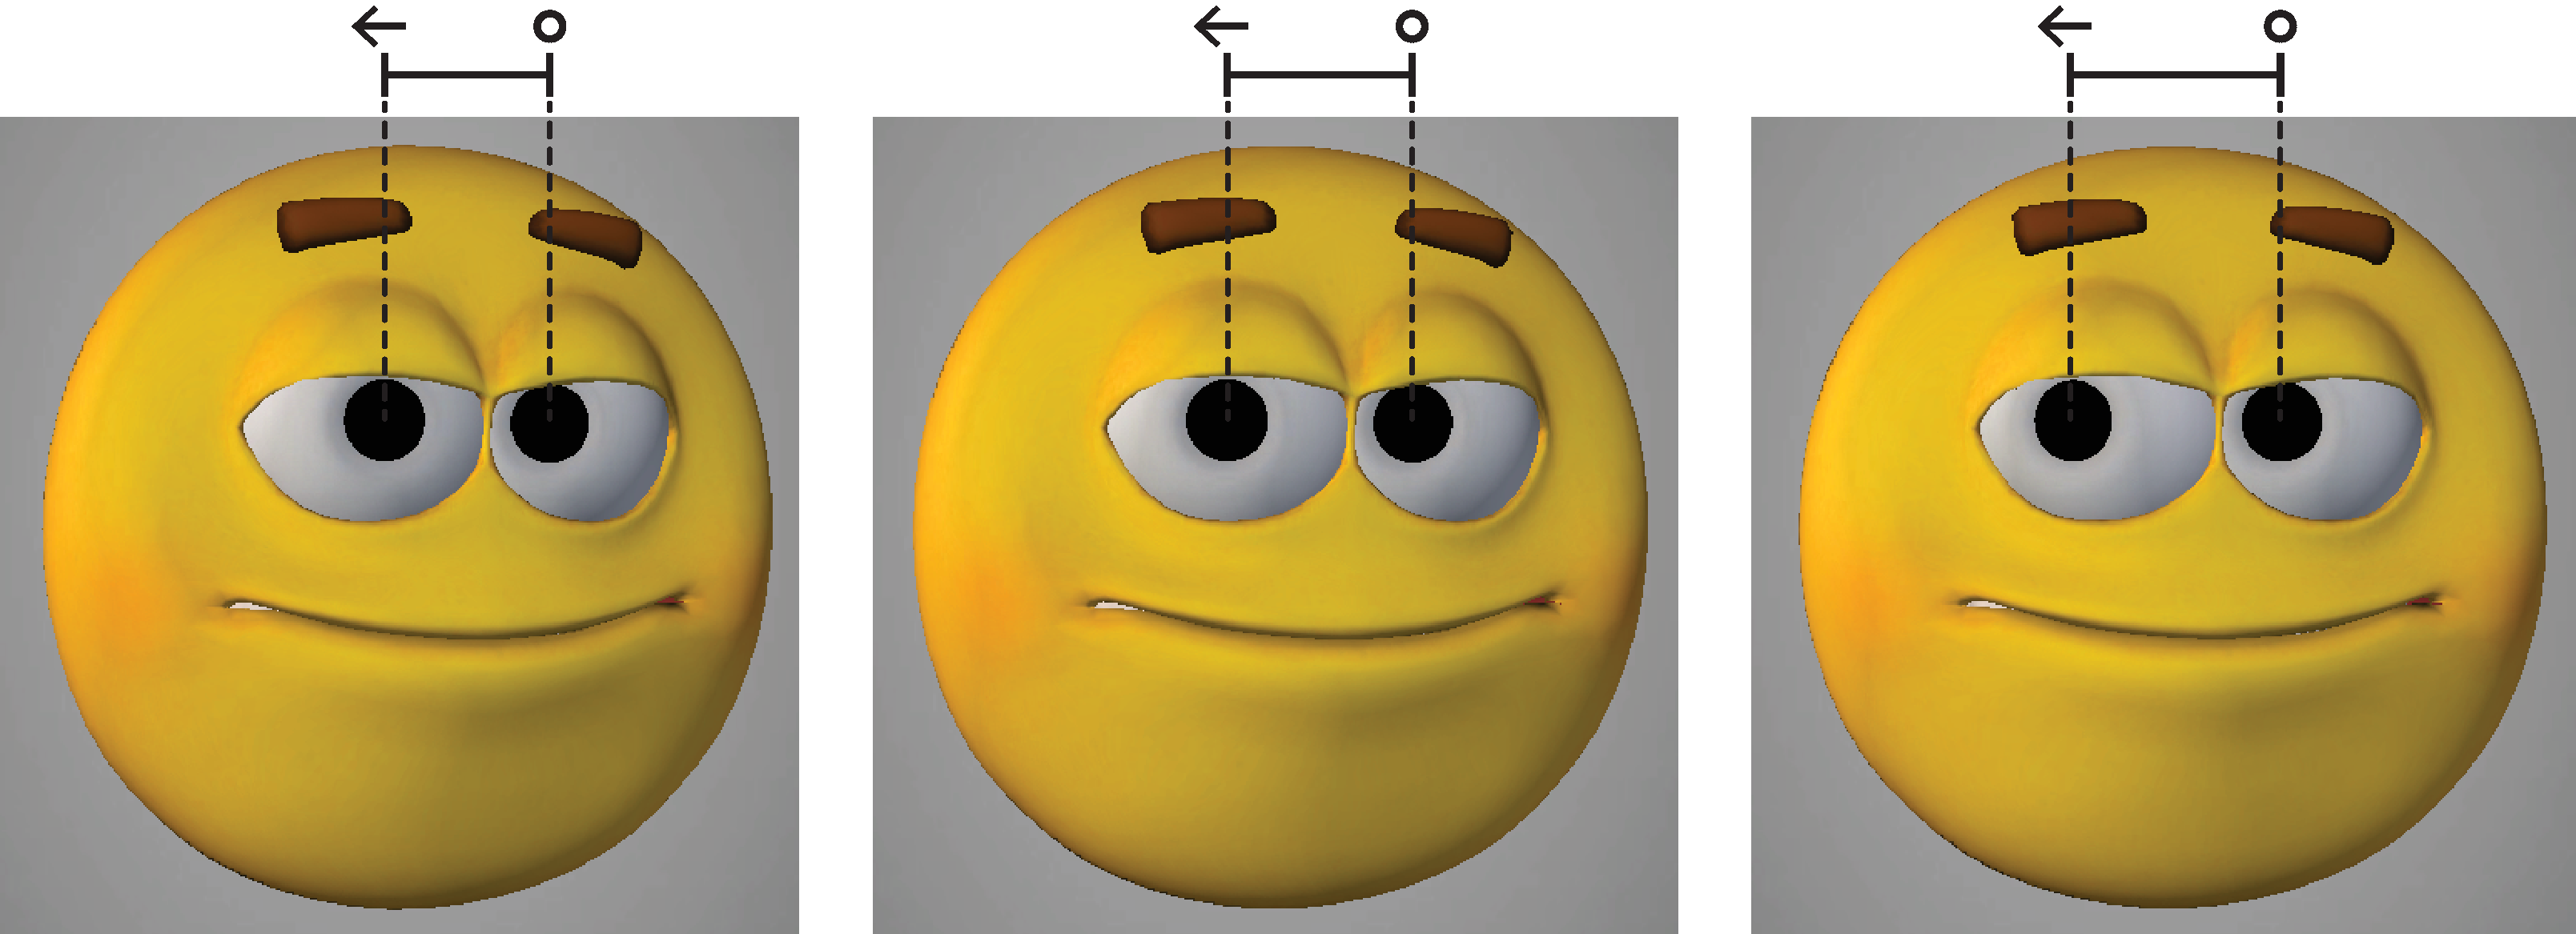
\includegraphics[width=0.75\textwidth]{figures/StuckEye.pdf}
\caption{Disconjugate eye movements due to asymmetric eye shape. The right eye is moving ahead,
while the left eye is blocked at OMR limit. Notation: Dot $\circ$ indicates that the left eye is stationary.}
\label{fig:StuckEye}
\end{figure*}

\subsection{Evaluation}

Stylized gaze techniques produce poses and movements that look \emph{plausible} by removing animation artifacts, and they do so in a \emph{robust} way, which means they should perform well on morphologically varied characters. To verify these claims, we performed a simulation where we synthesized a variety of gaze shifts across a range of characters and we quantitatively measured the prevalence of animation artifacts in these examples, finding that artifact prevalence is greatly reduced when using stylized gaze techniques.

Moreover, stylized gaze techniques depart from biomechanically valid human gaze, so we needed to verify whether this departure has any impact on the communicative function of gaze---i.e., whether attention direction is still accurately communicated following adaptation to a stylized character. We conducted a study where participants were shown videos of characters with realistic and stylized morphologies performing gaze shifts toward targets in the environment and asked to infer what target the character was gazing at. We found that adapted gaze shifts had the same accuracy as unadapted gaze on a realistically proportioned character, demonstrating that they remained \emph{effective}.
%In the same study, we asked the participants to rate the naturalness of gaze shifts in various conditions (using the same naturalness measure employed in~\citet{andrist2012headeye}) and  found no significant effect. This result suggests that gaze shift motion adapted by our techniques has the same \emph{plausibility} as unadapted gaze on a realistic character, but it also suggests that animation artifacts of unadapted gaze on a stylized character had no impact on plausibility that we could detect by the chosen measure.

\section{Authoring Plausible Directed Gaze (ongoing)}
\label{sec:GazeAuthoring}

The focus of my work is on animating gaze in scenarios involving a character performing some actions in a virtual environment---Figure~\ref{fig:PlausibleGazeAuthoring} shows two examples. With growing availability of low-cost, low-volume motion capture, such scenarios are becoming increasingly cost-effective to produce. However, this cost-effectiveness only extends to capturing body motion, while authoring gaze animation remains a challenge. Typical motion capture setup does not record eye movements (separate eye tracking technology is required for that purpose) and editing the character's gaze is frequently necessary to correct for errors in the performance and modify its content. My proposed solution is a gaze authoring approach that, given an input body motion and environment, automatically infers a directed gaze behavior that looks \emph{plausible}.

The basis of our authoring approach is a concise representation of directed gaze as a temporal sequence of \emph{gaze annotations} accompanying the original motion, where each annotation describes a gaze shift toward a target in the environment, followed by fixation of that target. Annotations specify only the basic timing and posture properties of the gaze shift while abstracting away motion details. Actual gaze shift kinematics are synthesized automatically by a gaze controller using our neurophysiology-based gaze shift model (Section~\ref{sec:GazeShifts}), which ensures that the resulting animation looks plausible given the specification. The representation based on gaze annotations forms the backbone of our gaze authoring system: we provide (1) methods for automated \emph{inference} of annotations from motion capture data, (2) an accessible graphical tool for manual \emph{editing} of the annotations, and (3) a robust approach for \emph{synthesis} of natural gaze movements from the annotation sequence:

\begin{enumerate}
\item \emph{Gaze inference} model infers a plausible directed gaze behavior for the given body motion and environment by analyzing the properties of the body motion signal. The model searches the motion signals of the head and torso joints for occurrences of the characteristic gaze shift kinematic profile (reported in~\citep{pejsa2015gaze}) to infer gaze shift timings, and it analyzes the facing direction of the head to infer the location of the likely gaze target in the environment. This inferred information is encoded in gaze annotations, from which the corresponding gaze animation is synthesized (item 3). Figure~\ref{fig:PlausibleGazeAuthoring}, left illustrates an example of adding inferred gaze to a captured body motion.
\item \emph{Gaze editing} tool enables modification of the gaze behavior by editing the annotations. Animator can use a graphical tool, implemented as an add-on for Unity game engine (Figure~\ref{fig:GazeEditingTool}), to add or remove gaze shifts toward specified targets, adjust gaze shift timings, fine-tune head and torso postures via alignment parameters, and edit gaze indirectly by editing the environment and gaze target layout. Figure~\ref{fig:PlausibleGazeAuthoring}, right shows an example of characters' gaze behaviors edited by adding gaze toward a new target.
\item \emph{Gaze synthesis} techniques generate gaze shift movements from the annotation sequence and layer them onto the character’s body motion. For each annotation, our gaze controller synthesizes a coordinated eye, head, and torso movement toward the specified gaze target. The synthesized movement is layered onto the body motion such that elements of the original body posture are preserved, and an inverse kinematics solver is employed to preserve end-effector constraints, which can become violated due to changes in torso posture effected by gaze. The result is a final character motion that incorporates the gaze behavior while preserving expressive properties and kinematic constraints of the original motion.
\end{enumerate}

\begin{figure*}
\centering
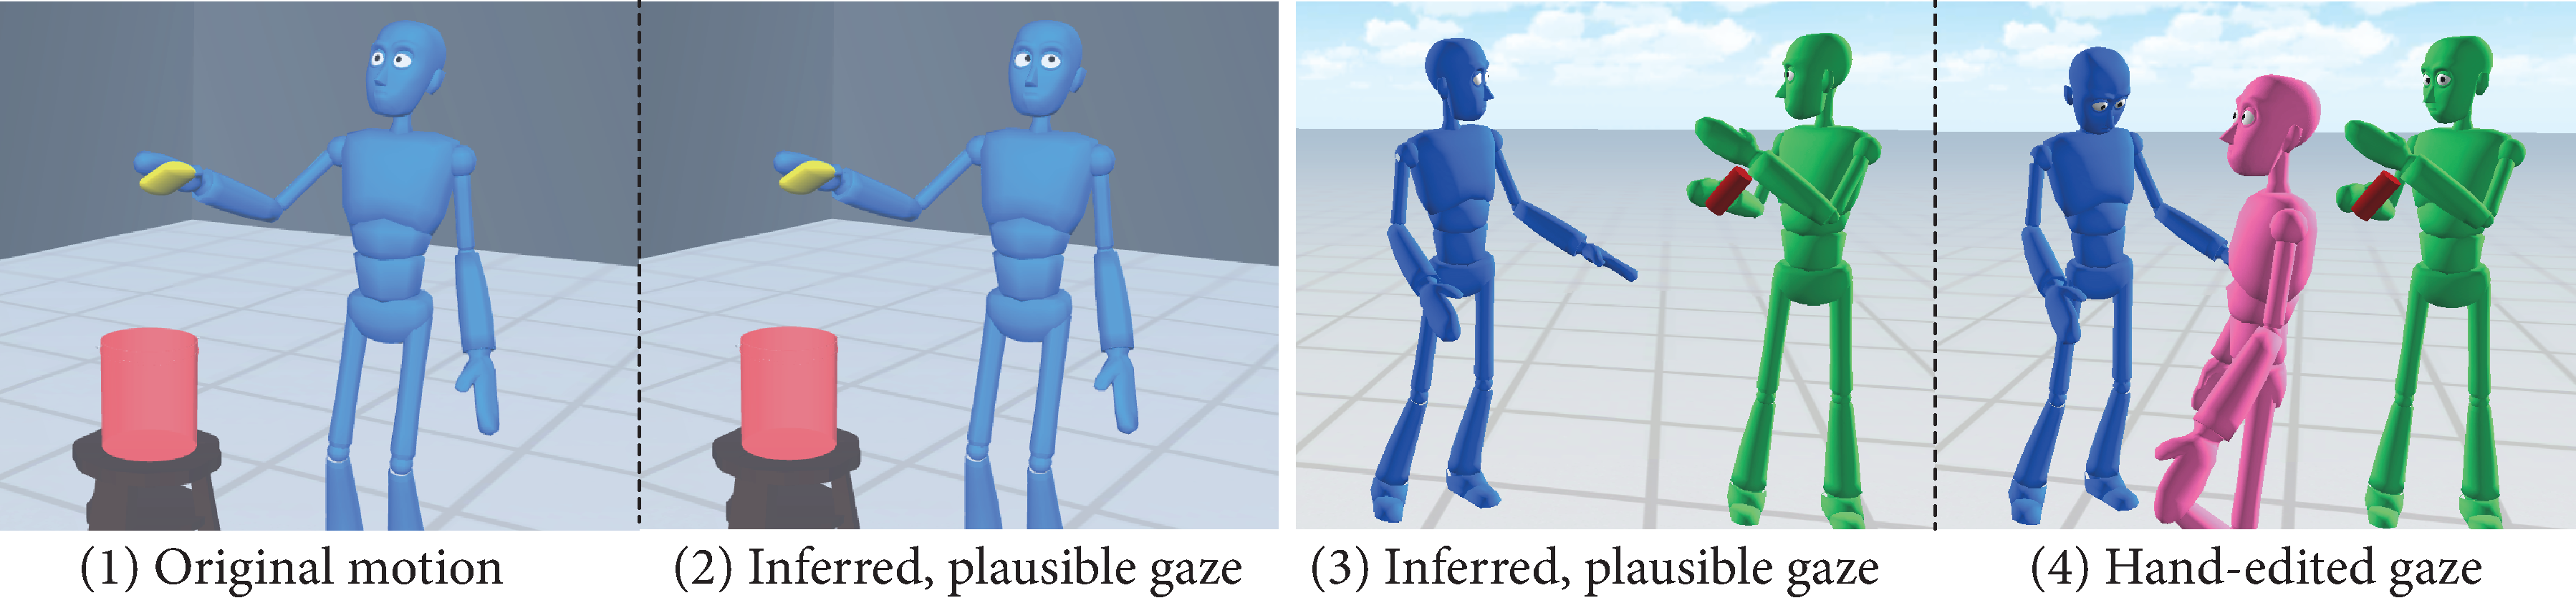
\includegraphics[width=1\textwidth]{figures/PlausibleGazeAuthoring.pdf}
\caption{Examples of directed gaze created using our approach for plausible gaze authoring. From left to right: (1) Original, captured body motion. (2) Our system has automatically inferred and added plausible gaze to the original motion. (3) Motion with plausible, unedited gaze. (4) Added gaze toward a new character using our editing tool.}
\label{fig:PlausibleGazeAuthoring}
\end{figure*}

\begin{figure*}
\centering
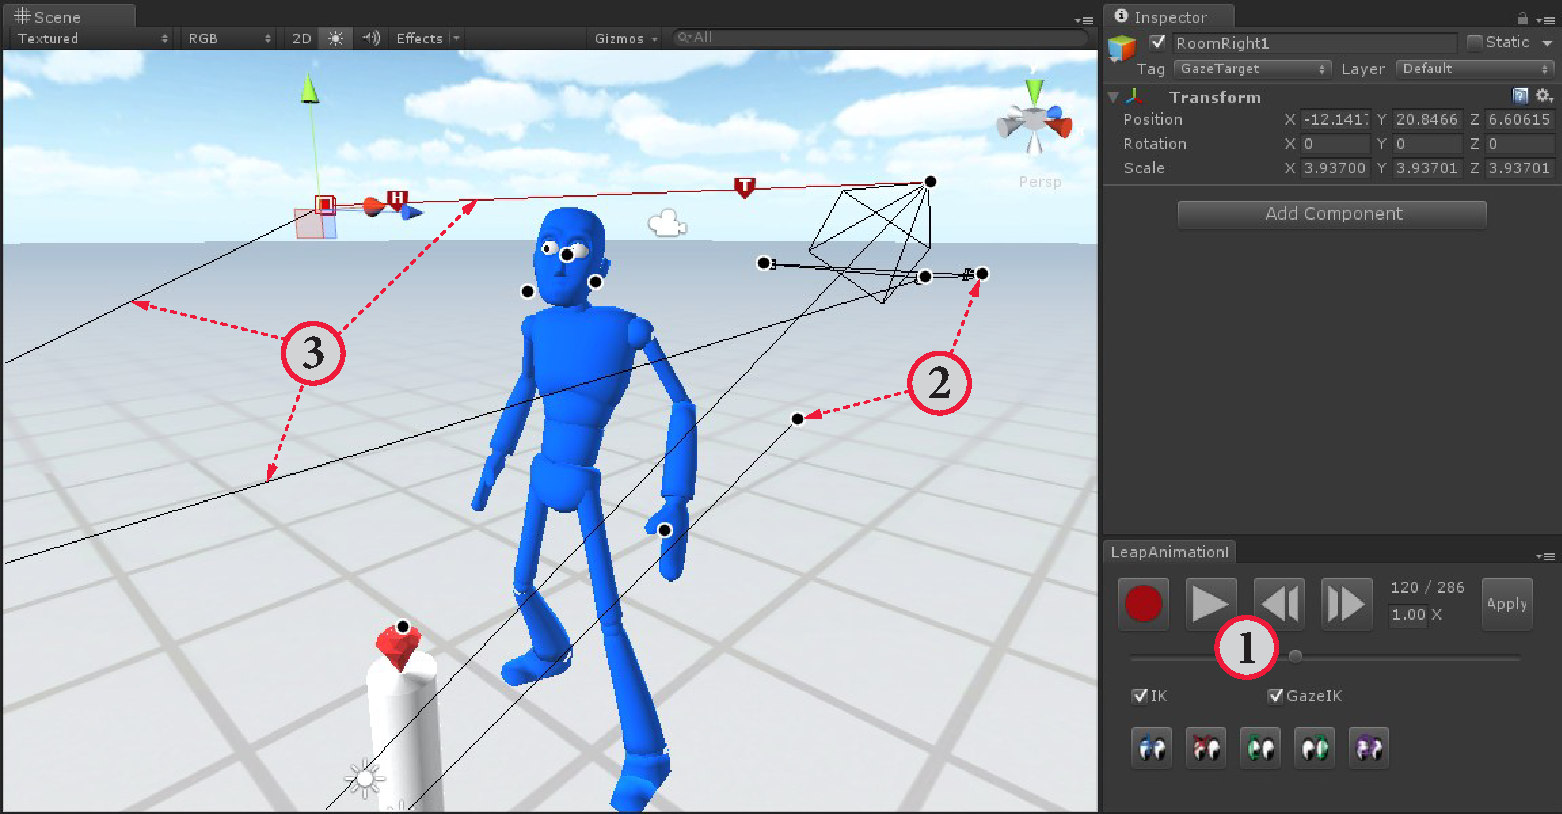
\includegraphics[width=1\textwidth]{figures/GazeEditingTool.pdf}
\caption{Graphical tool for hand-editing directed gaze. (1) Controls for animation playback and editing operations. (2) Dots indicate gaze targets in the virtual environment. (3) Directed lines connecting the targets represent gaze shifts.}
\label{fig:GazeEditingTool}
\end{figure*}

The directed gaze model supported in our approach is not a comprehensive model of human gaze. Real human gaze involves other types of movements, such as smooth pursuit, random saccades, and eye blinks. Smooth pursuit movements occur in specific situations, such as visual tracking of moving objects---while we presently have no plans to incorporate them, they have been computationally modeled in prior work~\citep{yeo2012eyecatch} and could be integrated in our system. However, eye blinks and random saccades occur constantly, so we have modeled them in our system (we use the Eyes Alive model for saccades~\citep{lee2002eyes}) and we generate them probabilistically as part of the synthesized gaze behavior. Eye blinks and saccades introduce non-deterministic variety into the otherwise deterministic directed gaze behavior and thus contribute to its plausibility.

\subsection{Evaluation}

We have demonstrated the gaze authoring approach on a range of scenarios, including multi-character interactions, walking around an environment, and complex environment interactions. To evaluate the \emph{cost-effectiveness} of the approach, we had an experienced animator author gaze animation in several scenarios using a traditional keyframing workflow and we measured the required effort as the number of required operations (set keyframes), which we compared to the number of operations used in our own tool. In one example, the animator had to set 143 keyframes to animate just the eyes, while our system could synthesize a similar estimate of eye movements completely automatically.

It still remains to conduct an evaluation of \emph{robustness} and \emph{plausibility} of the resulting gaze animation. One possible approach is to measure plausibility as overlap between inferred gaze behavior and some ground truth for a range of motions. Motions with hand-animated gaze could be used as ground truth or new motions could be captured while using an eye tracker to obtain their actual eye movements. Another approach is to measure plausibility in a study as participants' aesthetic preference for motions with inferred gaze. On each trial of the task, the participant would be shown two versions of the motion from a pool of three (original motion without gaze, motion with inferred gaze, motion with ground-truth gaze) and asked to choose which one they like better. Significant preference for inferred gaze over no gaze would be sufficient evidence of plausibility, further strengthened if there were no significant preference for ground-truth gaze over inferred gaze. Both studies need to be conducted with a large and varied pool of motions to also verify the \emph{robustness} of the approach.

\section{Authoring Effective Directed Gaze (planned)}
\label{sec:GazeBehaviorSynthesis}

The gaze authoring approach proposed in Section~\ref{sec:GazeAuthoring} can automatically produce gaze behavior that looks \emph{plausible}, but not \emph{effective}, because the inference model has no notion of communicative effects that the gaze behavior should trigger. To support such effects, the animator would need to use the manual editing tool to introduce specific gaze patterns into the original behavior. For example, to make the character's gaze more engaging, the animator would need to manually add gaze shifts toward the camera throughout the scenario. That is not the most \emph{cost-effective} approach, as the number of operations required increases linearly with scenario length, and a degree of expert knowledge is required, since the animator must know which gaze patterns yield the desired effects in communication. Ideally, it should be possible to have the animator specify the desired communicative effects once and then automatically synthesize the gaze patterns that achieve them. In this section, I discuss an extension to the gaze authoring approach that meets this objective.

%I will further augment the proposed authoring approach with a new automated synthesis model producing gaze behavior that is not only plausible for the current animated scenario, but also \emph{effective} given the animator-specified communicative goals. The model will expose a set of attention parameters enabling the animator to easily specify how the character should distribute its attention among the viewer and task objects, allowing automated synthesis of gaze patterns that optimize for effects such as improved engagement or understanding of task information.
I propose a new gaze inference model that accepts low-level inputs (body motion and environment, as well as a small set of high-level \emph{attention parameters}. The attention parameters will let the animator specify how the character should distribute its attention over the course of the interaction, allowing them to design a gaze behavior with specific effects on the viewer. One subset of parameters will be \emph{gaze posture parameters}, which will influence how the character distributes its head and body posture between the viewer and environment via the gaze shift model's head and torso alignment parameters. Another subset will be \emph{gaze pattern parameters}, which will control the probability of a particular gaze pattern, including: (1) \emph{affiliative gaze}, where the character predominantly looks at the viewer, potentially leading to greater engagement of the viewer and more positive perceptions of the agent; (2) \emph{referential gaze}, where the character alternates between looking at viewer and signaling their referential or action intent toward environment objects, resulting in potentially better recall of information grounded in those objects (Figure~\ref{fig:SandwichMaking}); (3) \emph{neutral gaze}, where the character focuses on the environment and does not gaze at the viewer at all.

\begin{figure*}
\centering
\includegraphics[width=1\textwidth]{figures/SandwichMaking.pdf}
\caption{Example scenario where the actor demonstrates the process of making a sandwich. Actor is displaying a gaze pattern characteristic of \emph{referential gaze}, consisting of gaze toward the viewer (left), followed by a gaze shift toward the next ingredient (middle) that grounds the linguistic reference to the ingredient and signals the intent to pick it up, and ending with a gaze shift back to viewer (right).}
\label{fig:SandwichMaking}
\end{figure*}

The new gaze inference model will compute a gaze behavior (expressed as a sequence of annotations) that is as close as possible fit to the given body motion, environment, and attention parameter values. The model could be implemented as a hill-climbing, state-space search, where states correspond to various gaze shift sequences describing the complete gaze behavior. The initial state for the search could be the output of the original gaze inference (using just the body motion and environment as inputs)---which we know to be a plausible gaze behavior---and neighboring solutions could be generated by probabilistically adding and removing gaze shifts and evaluating their fitness with respect to the body motion, environment, and attention parameter settings.

\subsection{Evaluation}

Evaluation of the complete gaze authoring approach will constitute a separate research contribution; I discuss it in the next section.

\section{Effective Directed Gaze for Virtual Demonstrators (planned)}
\label{sec:DemonstratorsGaze}

In the final project, I will apply the gaze authoring approach to a concrete application---animating directed gaze of virtual agents performing physical task demonstrations, such as assembly, repair, and operation of various devices and machinery. This project will serve as an evaluation of the \emph{effectiveness} of directed gaze synthesized by the approach and \emph{robustness} of the approach with respect to different attention parameter settings, and it will also constitute a larger contribution by informing the design of gaze behaviors for animated agents in an educational setting. Previous research has shown that virtual agents and social robots with appropriately designed gaze patterns can facilitate better information recall in scenarios such as storytelling~\citep{mutlu2006storytelling} and lecturing~\citep{andrist2012designing}. Findings from these studies suggest that increased gaze from the agent can lead to improved information recall and that head alignment during gaze has effects on information recall, engagement, and positive perceptions of the agent.

Designing the agent's gaze behavior in a physical task demonstration is challenging from the standpoint of authoring \emph{robustness} and \emph{cost-effectiveness}. Such a demonstration is likely to involve a lot of interaction with task objects in the environment. Appropriate gaze behavior in such scenarios will involve gaze toward relevant objects as they are discussed or handled by the demonstrator. On the other hand, the demonstrator should also gaze toward the viewer to make the demonstration more immediate and engaging, and to initiate joint attention toward important task objects. An effective virtual demonstration requires a complex interplay of gaze patterns that are difficult to author manually. Furthermore, this complex gaze behavior must be layered onto the complex, contact-rich body motion and adapted to the spatial layout of task objects. Prior studies of gaze tended to focus on storytelling and lecturing scenarios with little environment interaction and therefore simpler body motions and gaze patterns. Our gaze synthesis approach will be able to infer appropriate gaze patterns in an automated and therefore \emph{cost-effective} way, and it will be \emph{robust} to variation and complexity in body motion and environment layout. The application of the approach to the problem of virtual demonstrations will also serve as a demonstration of robustness and cost-effectiveness.

My proposed plan for the current research thread is to conduct a study with human participants to investigate the effects of the virtual demonstrator's gaze behavior on the effectiveness of their demonstration. We will devise model assembly and repair tasks---i.e., tasks designed to be mechanically  similar to real-world assembly and repair---and capture a human performing demonstrations of these tasks. A model assembly task might be constructing a specified shape out of toy blocks, while a model repair task might be correcting a mistake in a previously assembled shape. Next, we capture a demonstrator performing these tasks using a motion capture setup built for this purpose. For example, Figure~\ref{fig:SandwichMaking} illustrates an assembly task being captured with a markerless setup consisting of a pair of Kinect 2 devices and a head-worn eye tracker. Given the captured motion and a 3D model of the task environment, we will use our gaze authoring approach to synthesize the directed gaze animation to match the captured performance and reconstructed task environment. We will manipulate the gaze inference model's attention parameters to yield gaze behaviors designed to maximize viewer engagement (affiliative gaze) and task understanding (referential gaze). These gaze behavior variations will serve as distinct conditions in our study.

We will show the virtual demonstrations as stimuli to our participants and we will measure their effects on participants' (1) task understanding, (2) engagement, (3) perception of the demonstrator's credibility and competence, and (4) attention. To measure \emph{task understanding}, we will employ an objective measure, such as a questionnaire measuring information recall or having the participants perform the task and measuring completion time. For measuring \emph{engagement} and perceived \emph{credibility} and \emph{competence} we can employ previously validated subjective questionnaires from studies such as~\citep{andrist2012designing}. Finally, to truly explain how the agent's gaze patterns shape participants' understanding and subjective experience of the task, we must understand their effect on participants' \emph{attention} over the course of the demonstration---we can measure the latter by monitoring the participant's own gaze patterns using an eye tracker. 
%%% SOME OF THIS CODE IS ADAPTED FROM THE VENERABLE withesis.cls

%% BEGIN PAGESTYLE

%%% You can pick a pagestyle if you want; see the memoir class
%%% documentation for more info.  The default ``deposit'' option meets
%%% the UW thesis typesetting requirements but is probably
%%% unsatisfactory for making a version of your dissertation that
%%% won't be deposited to the graduate school (e.g. for web or a nice
%%% printed copy)

\chapterstyle{deposit}
\pagestyle{deposit}

\chapter{Conclusion and Expected Contributions}

The goal of my research is to make it easier for animators to produce directed gaze animation for virtual characters in a range of animated scenarios, such that the resulting gaze behavior looks plausible and is effective as a mechanism for communicating the character's attention to the viewer and directing the viewer's attention in a way that facilitates positive effects such as increased engagement and learning. My proposed approach for achieving this goal is a new authoring workflow based on a combination of automated inference and manual editing, which I will employ in the context of designing effective gaze behaviors for virtual agents performing physical task demonstrations.

Table~\ref{tab:overview} gives an overview of the work's components, how each component contributes to the four cornerstones of my thesis (plausibility, effectiveness, robustness, and cost-effectiveness), and how I plan to evaluate each contribution.

\bgroup
\def\arraystretch{1.5}
\begin{sidewaystable}
\caption{Overview of contributions and planned evaluations}
\label{tab:overview}
\tiny
\begin{tabularx}{\textwidth}{|p{2.7cm}||X|X|X|X|}
\hline
\textbf{Component} & \textbf{Plausible} & \textbf{Effective} & \textbf{Robust} & \textbf{Cost-effective} \\
\Xhline{2\arrayrulewidth}
\multirow{2}{*}{1. \emph{Gaze shift model}}
& Kinematics based on primate neurophysiology
& Target, head and torso alignment parameters
& \textcolor{red}{Not robust to character morphology}
& Intuitive parametrization, automatic timing \\
& Evaluation: head-eye model previously evaluated in~\citep{andrist2012headeye}
& Evaluation: (1) head-eye model previously evaluated in~\citep{andrist2012headeye} and~\citep{andrist2012designing}; (2) study measuring torso alignment effects on \emph{perceived interest} (level of attention)
& & Evaluation: see 3 and 4 \\
\hline
\multirow{2}{*}{2. \emph{Stylized gaze}}
& Removes artifacts on non-human character morphologies
& Retains the parametrization of the original model
& Works across a range of character morphologies
& See 1 \\
& Evaluation: (1) simulation measuring artifact prevalence; (2) study measuring \emph{communicative accuracy} and \emph{naturalness}
& Evaluation: study measuring \emph{communicative accuracy} and \emph{naturalness}
& Evaluation: as for plausibility, (1)
& \\
\hline
\multirow{2}{*}{3. \parbox{2.5cm}{\emph{Authoring plausible gaze}}}
& Plausible for body motion and environment; neurophysiology-based gaze shift model
& \textcolor{red}{Not cost-effective, requires manual editing to achieve specific gaze patterns}
& Works across a range of body motions and environments
& Get plausible results automatically, with optional use of an accessible manual editing tool \\
& Evaluation: (1) simulation measuring overlap with ground truth; (2) study measuring aesthetic preference for inferred gaze motions
& 
& Evaluation: as for plausibility
& Evaluation: comparison of effort required\\
\hline
\multirow{2}{*}{4. \parbox{2.5cm}{\emph{Authoring effective gaze}}}
& See 3
& Automated inference with attention parameters to achieve specific gaze patterns
& Works across a range of body motions, environments, and attention parameter settings
& Get effective results automatically \\
& 
& Evaluation: see 5
& Evaluation: see 5
& Evaluation: see 5 \\
\hline
\multirow{2}{*}{5. \parbox{2.5cm}{\emph{Effective gaze for virtual demonstrators}}}
& 
& Attention parameters set to obtain affiliative, referential, and neutral gaze patterns on a virtual demonstrator
& Task demonstrations have complex body motion, environment, and gaze patterns
& \\
& 
& Evaluation: study measuring the gaze effects on \emph{attention}, \emph{engagement}, \emph{task understanding}, and \emph{demonstrator credibility} and \emph{competence}
& Evaluation: production of study stimuli
& \\
\hline
\end{tabularx}
\end{sidewaystable}

%Expected contributions from this work are the following:
%\begin{enumerate}
%\item A procedural animation model for synthesis of directed gaze shifts as building blocks of the larger gaze behavior, with support for coordinated movement of the eyes, head, and torso.
%\item Stylized gaze techniques for adapting gaze shift motion to characters with non-realistic and non-human morphologies.
%\item An approach for authoring plausible directed gaze combining automated inference from body motion and environment with accessible manual editing.
%\item An extension of the approach with automated inference of effective gaze that achieves animator-specified communicative effects.
%\item A study of effective gaze for virtual demonstrators, that serves as an evaluation of the animation approach but also adds to the understanding of effective gaze behavior design for animated agents in an educational setting.
%\end{enumerate}
% TODO: some illustration of how my research projects build on each other:
% 1. Gaze shift, \alpha_H, \alpha_T
% 2. Gaze shift on multiple characters, \alpha_H, \alpha_T, \alpha_E
% 3. Sequence of gaze shifts, given body motion and environment
% 4. Sequence of gaze shifts, given body motion, environment, and high-level goals
% 5. Application of 4. to a specific domain 

%% Do you have appendices?  If so, add them here, just like chapters.
% \begin{appendices}
% \include{backmatter/appendix1}
% \end{appendices}

%% Are you a big nerd with a colophon?  Add it here.
%\begin{colophon}
%\svnidlong{$LastChangedBy$}{$LastChangedRevision$}{$LastChangedDate$}{$HeadURL: http://freevariable.com/dissertation/trunk/frontmatter.tex $}
\vcinfo{}

This template uses Gyre Pagella by default.  (I used Arno Pro in my dissertation.)

Feel free to give me a shout-out in your colophon or acks if this template is useful for you.  Good luck!

%\end{colophon}

%% McBride is a very nice style (some version is included in this distribution)
\bibliographystyle{mcbride}
\bibliography{refs}

%% Want an index?  Neither did I.
%\printindex

\end{document} 